\chapter{Planificación y costes} \label{chap:planificacionycostes}
El primer paso, una vez que hemos esbozado la idea del proyecto que tenemos entre manos, consiste en realizar una planificación detallada en la que establezcamos y definamos de manera precisa las tareas necesarias para abordarlo teniendo en cuenta todos los aspectos que pueden influir en el correcto desarrollo del mismo.

Para lograr la implantación de nuestra cloud y dar así un servicio de IaaS, tenemos que pasar por diversas fases de desarrollo que comentaremos en el siguiente punto. Además, se necesita de una planificación temporal que acompañe a las tareas y que veremos también en este capítulo.

No podemos olvidar los recursos necesarios para la elaboración del proyecto tanto humanos, como hardware,  software y servicios. Estos recursos se han escogido, en ocasiones, basándonos en el uso de los mismos durante la realización de los estudios de Grado.

Finalmente concluiremos este punto con un desglose del coste estimado de los distintos elementos del proyecto de los que iremos hablando a lo largo del capítulo y que darán un coste final total como colofón.


\section{Fases de desarrollo}
En esta sección vamos a listar todas las tareas que se van a llevar a cabo, agrupándolas en distintas fases y acompañándolas de una pequeña descripción. 

Las distintas fases de desarrollo junto las tareas de las que se componen, así como las fechas de inicio y fin y el número de días empleado para cada una se muestran en la Fig.\ref{fig:tareas}. Como se puede apreciar existe una clara relación entre las tareas y la estructura de la memoria \ref{subchap:estrucutramemoria}. Además tenemos los correspondientes diagramas de Gantt que muestran la contemporización de tareas por meses, en la Fig.\ref{fig:ganttMes} y para una mejor visualización por trimestres en la Fig.\ref{fig:gantTrimes}. 

En estas figuras podemos ver que la duración estimada del proyecto en días laborales desde que se inicia la primera tarea hasta que finaliza la última, entre las cuales está planificada la realizarán algunas tareas en paralelo, hacen un total de 223 días, de los cuales se estima un trabajo de de 3 horas diarias en días laborales, lo cuál tendremos en cuenta en el apartado \ref{subchap:costeshumanos} de costes humanos .

\begin{figure}
    \centering
    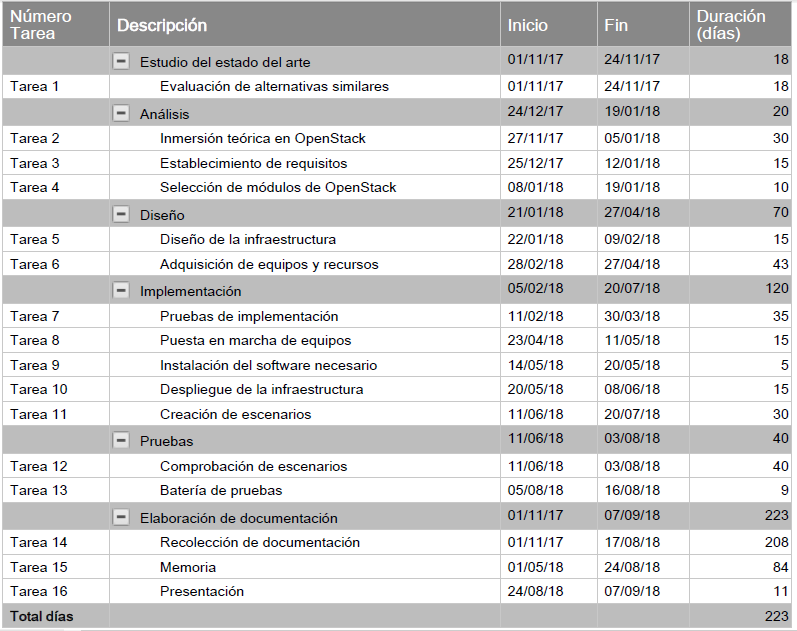
\includegraphics[width=1\textwidth]{imagenes/capitulo3/tareas.png}
    \caption{Planificación de tareas.}
	\vspace{0.3cm}
    \label{fig:tareas}
\end{figure}

\begin{figure}
    \centering
    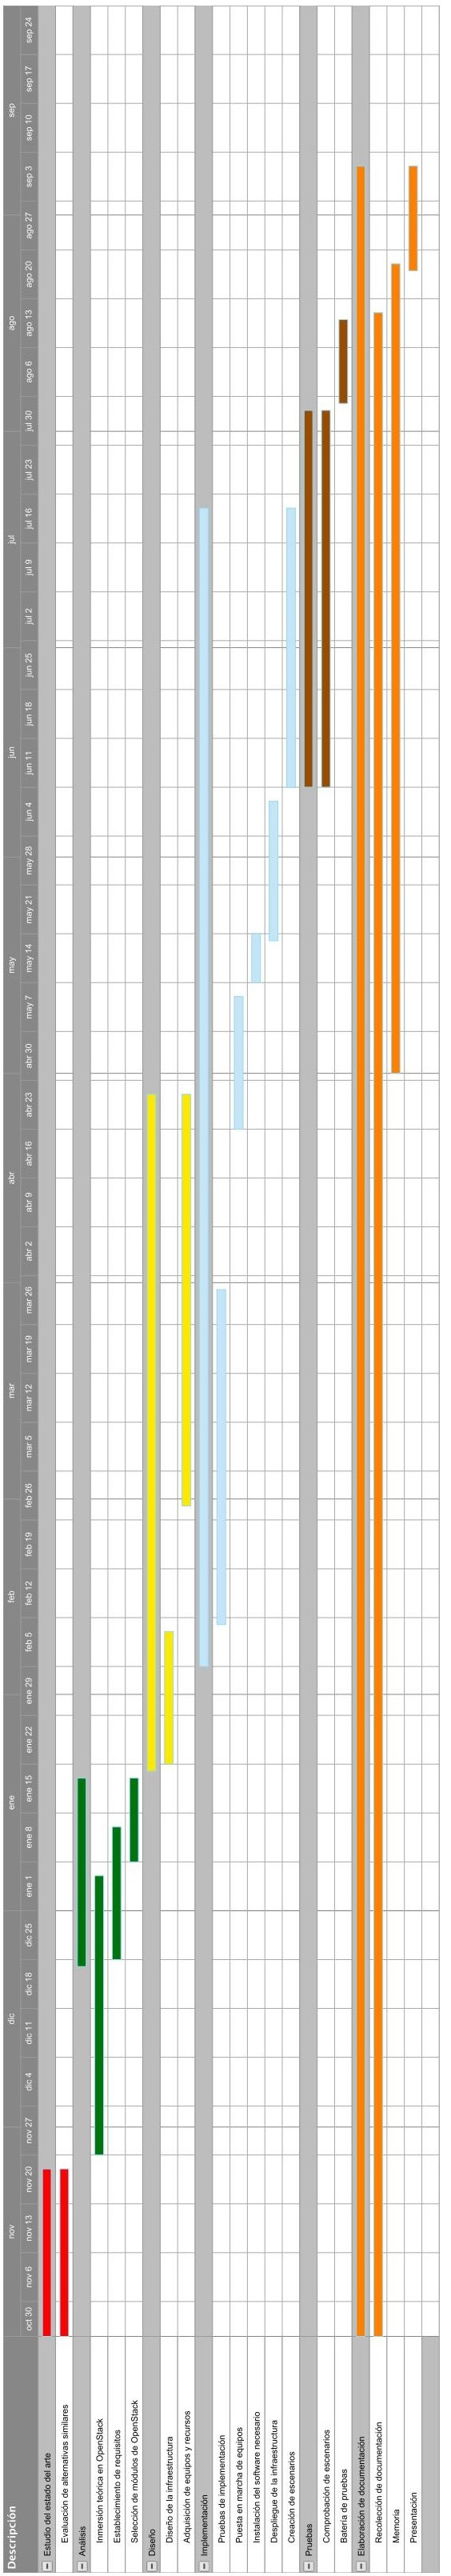
\includegraphics[width=0.32\textwidth]{imagenes/capitulo3/0001.jpg}
    \caption{Diagrama de Gantt mensual.}
	\vspace{0.3cm}
    \label{fig:ganttMes}
\end{figure}


\begin{figure}
    \centering
    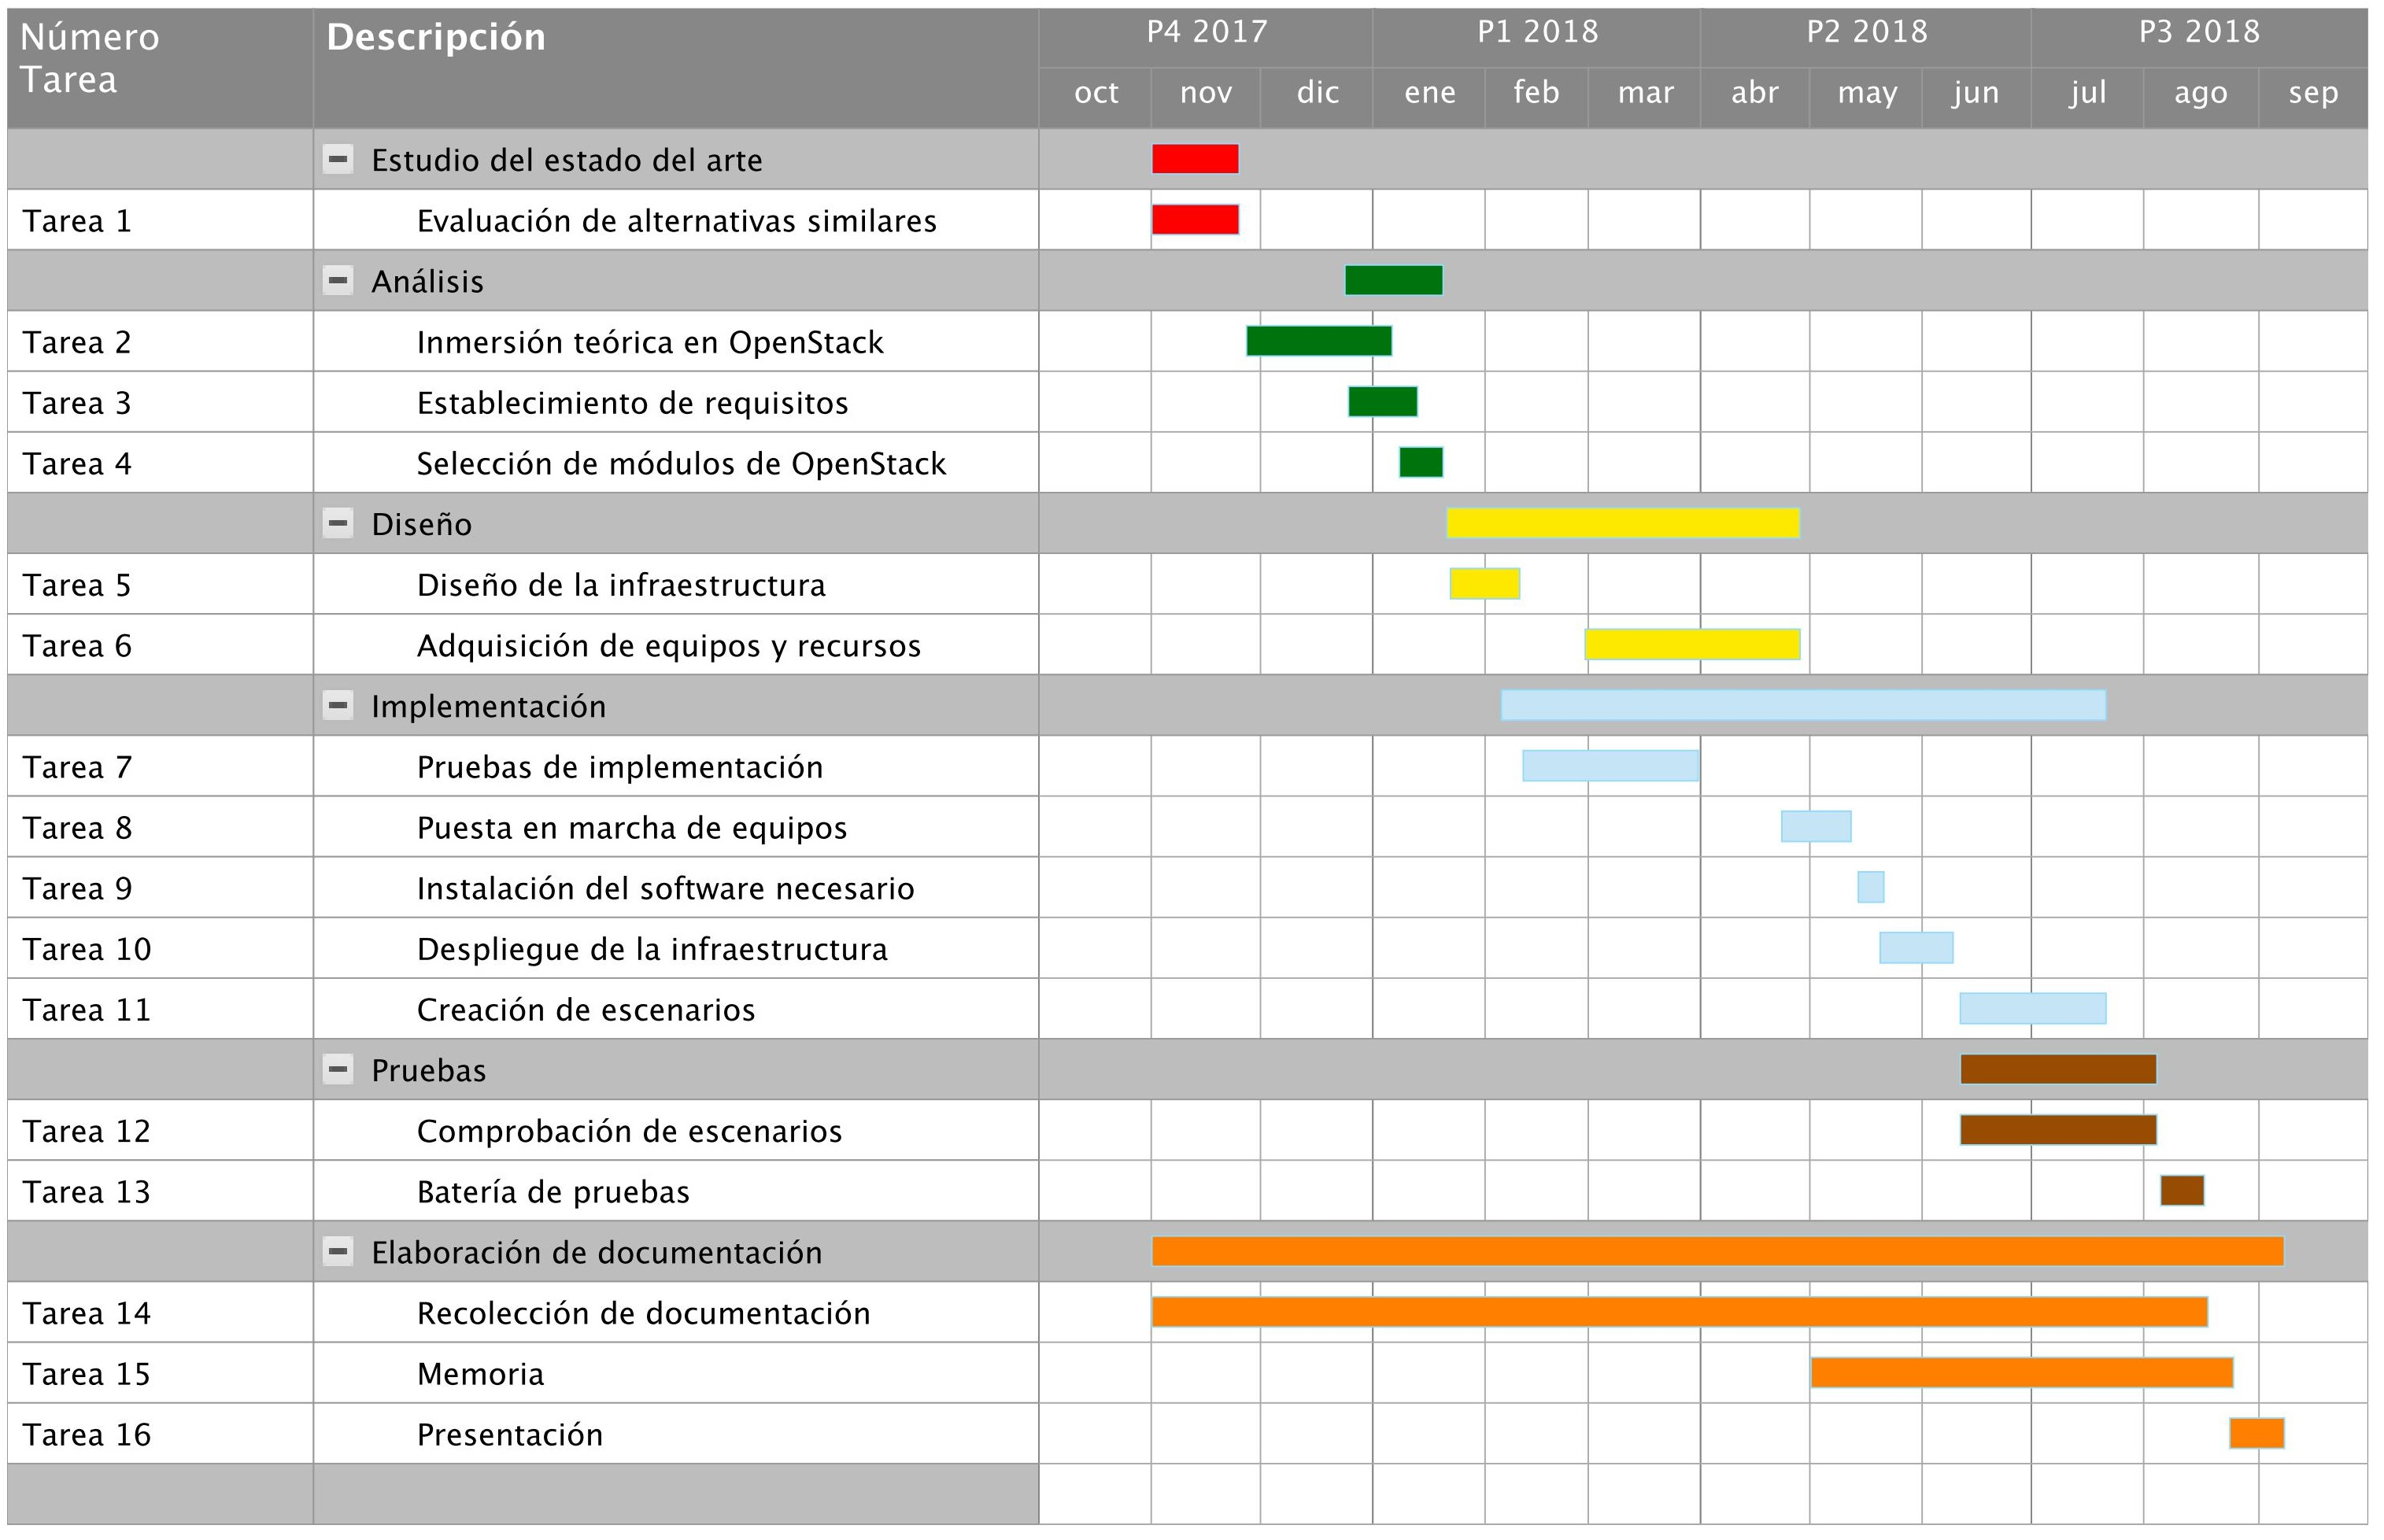
\includegraphics[width=1\textwidth]{imagenes/capitulo3/gantt-trimestral.jpg}
    \caption{Diagrama de Gantt trimestral.}
	\vspace{0.3cm}
    \label{fig:gantTrimes}
\end{figure}


\subsection{Estudio del estado del arte}
Dentro de esta primera fase, se evaluarán distintas alternativas similares a OpenStack para determinar si es la herramienta idónea para abordar el proyecto.

\subsection{Análisis}
Esta fase de análisis es vital, ya que nos servirá par adquirir un conocimiento profundo de OpenStack a nivel teórico así como definir los requisitos que necesitaremos para llevar a buen puerto este proyecto.

Una vez realizadas estas tareas tendremos el nivel necesario para decidir que módulos de OpenStack necesitamos instalar para poder gestionar métricas, alarmas, orquestación de funciones de red y otros.

En la memoria, el resultado de este apartado se ve reflejado a lo largo de todos los capítulos en los que se analizan distintos temas en función del apartado en el que nos encontremos.

\subsection{Diseño}
Ya definida la planificación de los requisitos, especificaciones y  módulos a estudiar para nuestro entorno IaaS, podemos diseñar la infraestructura de red que soportará nuestro servicio a nivel teórico.

En esta fase y en paralelo se irán adquiriendo los recursos hardware y software que necesitaremos tras el estudio de la fase anterior.

\subsection{Implementación}
Con todo a punto, en esta fase nos pondremos a desplegar el entorno con el que trabajaremos en OpenStack. Para ello en primer lugar se realizarán una serie de pruebas de instalación e implementación en un ordenador personal para una vez puesta en marcha los distintos equipos necesarios, poder instalar el software de OpenStack y realizar el despliegue de la infraestructura sea una tarea más ágil y precisa.

En este apartado se crearán también los distintos escenarios que justifican la elaboración de esta memoria.


\subsection{Pruebas}
El despliegue de la infraestructura finalizará con la comprobación del correcto funcionamiento de los distintos escenarios planteados en los que se harán una serie de pruebas para asegurarnos de que el entorno creado se comporta de acuerdo a las necesidades de orquestación de funciones de red que tenemos.

\subsection{Documentación}
Esta última fase comienza desde el principio de la elaboración del proyecto. Por un lado desde el inicio hasta prácticamente el final del proyecto se irá recolectando información y fuentes que iremos necesitando para superar las distintas fases aquí explicadas.

Se incluye aquí la realización tanto de la memoria técnica como de la presentación para la defensa final que se expondrá ante el jurado.

\section{Recursos}
En esta sección se hará un desglose en distintas subsecciones de los recursos que puedan estar implicados en este proyecto, tanto humanos como de hardware y software, facilitando así la estimación de costes en la sección posterior.

\subsection{Recursos humanos}
Los recursos humanos de este proyecto serán las personas implicadas en el mismo, a saber:

\begin{itemize}
\item D. Jorge Navarro Ortiz. Profesor titular de universidad del departamento de \textit{Teoría de la señal, telemática y comunicaciones} de la \textit{Universidad de Granada}. Tutor del presente trabajo fin de grado.
\end{itemize}

\begin{itemize}
\item Alejandro Toledo Juan. Estudiante del \textit{Grado en Ingeniería de Tecnologías de Telecomunicación} en la \textit{Escuela Técnica Superior de Ingenierías Informática y de Telecomunicación}, \textit{Universidad de Granada}. Autor del presente trabajo fin de grado.
\end{itemize}


\subsection{Recursos hardware}
Para la implementación del proyecto se requerirán los siguientes recursos hardware:
\begin{itemize}
\item Ordenador portátil Sony Vaio PCG-81112M con procesador Intel Core i7-4710HQ a 2,5 GHz, con una memoria RAM de 8 GB y disco duro de 500 GB. Este portátil será utilizado para la realización de pruebas de implementación de OpenStack antes de la instalación definitiva en los servidores.
\item Servidor 1. Asus G11 CD-K-SP012T. Procesador Intel Core i7-7700 a 3,6 GHz, con una RAM de 16 GB DDR4 y disco duro de 1TB más 128 GB SSD SATA3. Este servidor será el principal a la hora del desarrollo e implementación de nuestra nube.
\item Servidor 2. Acer G3-710. Procesador Intel Core i7-7700 a 3,6 GHz, con memoria RAM de 32 GB y disco duro de 1TB más 256 GB SSD. En este servidor se creará la segunda región de nuestra cloud que simulará un data center localizado en otro emplazamiento geográfico.
\item TP-LINK DGE-Tarjeta de Red Gigabit 10/100/1000. Tarjeta de red que se instalará en el segundo servidor para poder conectarse a Internet y permitir la conexión externa a través del primer servidor, ya que sólo dispondremos de una IP pública.
\item Cable RJ-45 Cat.5e. NANOCABLE: RJ45, Cat.5e UTP AWG24, latiguillo de 20 mts. Cable de red con latiguillo incluido de categoría 5e que usaremos para conectar los servidores entre sí y uno de ellos, el primero, a la toma de red que nos dará conexión a Internet.
\item Regleta APC P5BV-SP Regleta con Proteccion 5 Tomas y Coaxial 230V. Regleta que usaremos para conectar la alimentación de los servidores a la toma eléctrica.
\end{itemize}

\subsection{Recursos software}
Del mismo modo, he aquí el listado del software necesario para el desarrollo del TFG.
\begin{itemize}
\item Sistema operativo Ubuntu Server 16.04 LTS. Se ha optado por este sistema ya que es el aconsejado por los creadores de OpenStack para realizar la instalación all-in-one con Devstack y por el uso habitual del mismo durante el Grado y a nivel personal.
\item Openstack. El software necesario para la instalación de todos los componentes necesarios lo encontramos en los  repositorios de GitHub de all-in-one Devstack.\cite{noauthor_devstack:_2018}
\item Overleaf. Procesador de textos online gratuito basado en LATEX que usaremos para la redacción de la memoria.
\item Zotero. Herramienta para la gestión de referencias bibliográficas.
\item Smartsheet. Es un software online que nos permite diseñar diagramas de Gantt en distintos formatos.
\item Lucidchart. Esta herramienta disponible online, nos permite realizar todo tipo de diagramas: diagramas de red, diagramas de flujo, esquemas, diagramas UML...
\end{itemize}

\section{Estimación de costes}

\subsection{Costes humanos}\label{subchap:costeshumanos}
Actualmente en España no existe un salario de referencia para un profesional del sector\cite{noauthor_boe.es_nodate}, por tanto la estimación que aparece en la tabla \ref{tab:coste-recursos-humanos} se ha realizado en base a lo que suele cobrar un ingeniero de telecomunicaciones en función de su experiencia. Así, el precio por hora del trabajo en el proyecto realizado por Alejandro Toledo Juan, será de 20 \euro/hora mientras que el realizado por D.Jorge Navarro Ortiz y que se corresponde con las tutorías será de 50 \euro/hora. 

\renewcommand\arraystretch{1.1}
\begin{table}[!h]
\centering
\begin{adjustbox}{max width=\textwidth}
\begin{tabular}{|c|l|c|l|c|}
\hline
\textbf{Concepto} & \textbf{Precio/hora} & \textbf{Horas} & \textbf{Total}   \\
\hline \hline
Trabajo en el proyecto & 20 \euro/hora & 669 & 13380 \euro \\
\hline
Tutorías & 50 \euro/hora & 14 & 700 \euro \\
\hline
\multicolumn{3}{|l|}{\textbf{Total}} & \textbf{14080 \euro} \\
\hline
\end{tabular}
\end{adjustbox}
\caption{Estimación de costes de recursos humanos.}
\label{tab:coste-recursos-humanos}
\end{table}


\subsection{Costes hardware}
En la tabla \ref{tab:costes-hardware} se muestra un desglose de los costes de los recursos hardware. Para el coste de los servidores y el PC, se ha tenido en cuenta que el tiempo de vida útil está en torno a los 4 años, es decir, 48 meses. Se estima pues el coste de estos en el proyecto calculando la parte proporcional de ese coste para 5 meses que será el tiempo que se estima estén operativos:

Precio total del PC Portátil: 783.49\euro. Precio proporcional: 81.16\euro.
Precio total del Servidor 1: 1132.78\euro. Precio proporcional: 117.99\euro.
Precio total del Servidor 2: 1542.59\euro. Precio proporcional: 160.69\euro.
\renewcommand\arraystretch{1.1}
\begin{table}[!h]
\centering
\begin{adjustbox}{max width=\textwidth}
\begin{tabular}{|c|l|c|l|c|}
\hline
\textbf{Concepto} &  \multicolumn{1}{|c|}{\textbf{Descripción}} & \textbf{Cantidad}  & \textbf{Precio (\euro)}  \\
\hline \hline
PC Portátil & Sony Vaio: i7, 8 GB RAM  & 1 & 81.16 \\
\hline
Servidor 1 & Asus: i7, 16 GB RAM & 1 & 117.99 \\
\hline
Servidor 2 & Acer: i7, 32 GB RAM & 1 & 160.69 \\
\hline
Tarjeta Ethernet & TP-LINK DGE-Tarjeta de Red Gigabit 10/100/1000
 & 1 & 12.26 \\
\hline
Cable RJ-45 Cat.5e & NANOCABLE: RJ45, Cat,5e UTP AWG24, latiguillo de 20 mts
 & 2 & 13.56 \\
\hline
Regleta & APC P5BV-SP Regleta con Protección 5 Tomas y Coaxial 230V
 & 1 & 15.99 \\
\hline
\multicolumn{3}{|l|}{\textbf{Total}} & \textbf{402.11} \\
\hline
\end{tabular}
\end{adjustbox}
\caption{Estimación de costes de recursos hardware.}
\label{tab:costes-hardware}
\end{table}


\subsection{Costes software}
Como podemos ver en la tabla \ref{tab:costes-software} Todas las tecnologías que se pretenden usar en el proyecto están licenciadas bajo una licencia Open Source y por tanto no tienen ningún coste asociado.

\renewcommand\arraystretch{1.1}
\begin{table}[!h]
\centering
\begin{adjustbox}{max width=\textwidth}
\begin{tabular}{|c|l|c|l|c|}
\hline
\textbf{Concepto} &  \multicolumn{1}{|c|}{\textbf{Descripción}} & \textbf{Cantidad}  & \textbf{Precio (\euro)}  \\
\hline \hline
Sistema Operativo & Ubuntu Server 16.04 LTS
  & 3 & 0 \\
\hline
Openstack & All-in-one Devstack & 3 & 0 \\
\hline
Overleaf & Procesador de texto en LATEX online & 1 & 0 \\
\hline
Zotero & Gestor de referencias bibliográficas & 1 & 0 \\
\hline
Smartsheet & Diseño de diagramas de Gantt & 1 & 0 \\
\hline
Lucidchart & Diseño de diagramas  & 1 & 0 \\
\hline
\multicolumn{3}{|l|}{\textbf{Total}} & \textbf{0} \\
\hline
\end{tabular}
\end{adjustbox}
\caption{Estimación de costes de recursos software.}
\label{tab:costes-software}
\end{table}

\subsection{Costes de servicios}
Además de los costes ya citados, existen otros derivados de los servicios necesarios para el desarrollo de este trabajo y que tienen que entrar también en la planificación de gastos. Estos aparecen en la tabla \ref{tab:costes-servicios}. 

Vamos ahora a justificar la estimación de los mismos:

\begin{itemize}
\item Como podemos ver en la Fig.\ref{fig:tareas}, la puesta en marcha de los equipos comenzará el 23/04/18. En la puesta en marcha se contempla la solicitud de acceso al aula donde se han alojarán los equipos, de la IP pública necesaria para el acceso externo y la propia solicitud de los equipos hasta su posterior recepción. Se prevé disponer de los equipos ya instalados el 11/05/2018.

La desinstalación de la infraestructura  una vez finalizado el proyecto y la presentación, está planificada para el 14/07/2018. Esto hace un total de 127 días, o bien, 3048 horas.

En la tabla \ref{tab:costes-servicios} se ha calculado el precio de la luz teniendo en cuenta que el 11/05/2017, un año antes en la misma fecha que se prevé estén instalados los servidores, el precio medio de 1kWh era de 0.09808\euro/kW en Endesa.\cite{noauthor_endesa_nodate}

Mencionar que el precio se ha estimado en base al pico de potencia consumido por lo que será previsiblemente menor al que aparece.

\item Línea de acceso a Internet, que será la que nos permita la conexión remota y el acceso a la red externa en el entorno creado. La línea tiene un coste de 30\euro/mes y estará disponible durante 5 meses.
\end{itemize}


\renewcommand\arraystretch{1.1}
\begin{table}[!h]
\centering
\begin{adjustbox}{max width=\textwidth}
\begin{tabular}{|c|l|c|l|c|}
\hline
\textbf{Concepto} &  \multicolumn{1}{|c|}{\textbf{Descripción}} & \textbf{Consumo total(kW/h)}  & \textbf{Precio (\euro)}  \\
\hline \hline
Consumo energético & 2 servidores de 150 W  & 914.4 & 89.68\\
\hline
Internet & Línea de acceso durante 5 meses a 30\euro/mes &  & 150  \\
\hline
\multicolumn{3}{|l|}{\textbf{Total}} & \textbf{239.68} \\
\hline
\end{tabular}
\end{adjustbox}
\caption{Coste estimado de los servicios.}
\label{tab:costes-servicios}
\end{table}


\section{Presupuesto final}
\renewcommand\arraystretch{1.1}
\begin{table}[!h]
\centering
\begin{adjustbox}{max width=\textwidth}
\begin{tabular}{|c|l|}
\hline
\textbf{Concepto} & \textbf{Precio (\euro)}  \\
\hline \hline
Recursos humanos &  14080 \\
\hline
Recursos hardware & 402.11  \\
\hline
Recursos software & 0 \\
\hline
Servicios & 239.68 \\
\hline
\textbf{Total} & \textbf{14721.79} \\
\hline
\end{tabular}
\end{adjustbox}
\caption{Presupuesto final estimado.}
\label{tab:costes-final}
\end{table}

Una vez identificados todos los recursos que se van a utilizar y lo costes asociados a estos, podemos hacer un presupuesto final en el que aparecen todos ellos \ref{tab:costes-final}.

\jorge{Ten cuidado que te sales del margen}

Finalmente vemos que el coste total estimado del proyecto es de \textbf{14721.791\euro}, CATORCE MIL SETECIENTOS VEINTIUNO CON SETENTA Y NUEVE EUROS.